%%%%%%%%%%%%%%%%%%%%%%%%%%%%%%%%%%%%%%%%%%%%%%%%%%%
%% LaTeX book template                           %%
%% Author:  Amber Jain (http://amberj.devio.us/) %%
%% License: ISC license                          %%
%%%%%%%%%%%%%%%%%%%%%%%%%%%%%%%%%%%%%%%%%%%%%%%%%%%

\documentclass[a4paper,11pt]{book}
\usepackage[T1]{fontenc}
\usepackage[utf8]{inputenc}
\usepackage{lmodern}


%%%%%%%%%%%%%%%%%%%%%%%%%%%%%%%%%%%%%%%%%%%%%%%%%%%%%%%%%
% 
%%%%%%%%%%%%%%%%%%%%%%%%%%%%%%%%%%%%%%%%%%%%%%%%%%%%%%%%%
\usepackage{hyperref}
\hypersetup{
    colorlinks=true,
    linkcolor=DarkRed,
    filecolor=magenta,      
    urlcolor=green,
    pdftitle={Fernando Pujaico Rivera},
    bookmarks=true,
}

\usepackage{graphicx}
\usepackage{subcaption}
\usepackage[english]{babel}
\usepackage{amsmath,amsfonts,amsthm} % Math packages
\usepackage[svgnames]{xcolor} % Enabling colors by their 'svgnames'
\usepackage{comment}

\usepackage[left=2.5cm,right=2.5cm,top=2.5cm,bottom=2.5cm]{geometry}

\usepackage{biblatex}
%\addbibresource{section1.bib}




%% ARCMIN
%%\newcommand{\argmin}[1]{{\operatorname{arg}_{#1}\operatorname{min}}\;}

%% morepenrose function
\newcommand{\getminparam}{\operatorname{get}\_\operatorname{poly2}\_\operatorname{coefs}}

%% diagonal function
\newcommand{\funcdiag}{diag}


%% vectorization function
\newcommand{\funcvec}{vec}

%% transpose function
\newcommand{\funcinv}{inv}

%% transpose function
\newcommand{\functrans}{trans}
%% transpose operator
\newcommand{\transpose}{\mathrm{T}}

%% Time of sampling
\newcommand{\ToS}{\tau}

%% block matrix
%\newcommand{\funcblockdiag}{blkdiag}
%\newcommand{\funcblockhor }{blkhorz}
%\newcommand{\funcblockver }{blkvert}


%% definiçao de tipos de arrays
\newcommand{\TRIX}[1]{\mathbf{\overline{\uppercase{#1}}}}
\newcommand{\MATRIX}[1]{\mathbf{\uppercase{#1}}}
\newcommand{\VECTOR}[1]{\mathbf{\lowercase{#1}}}
\newcommand{\DTVECTOR}[1]{\mathbf{\dot{\lowercase{#1}}}}
\newcommand{\DDTVECTOR}[1]{\mathbf{\ddot{\lowercase{#1}}}}
\newcommand{\DDDTVECTOR}[1]{\mathbf{\dddot{\lowercase{#1}}}}
\newcommand{\DDDDTVECTOR}[1]{\mathbf{\ddddot{\lowercase{#1}}}}
%%%%%%%%%%%%%%%%%%%%%%%%%%%%%%%%%%%%%%%%%%%%%%%%%%%%%%%%%%%%%%%%%%%%%%%%%%%%%%%%
%%%%%%%%%%%%%%%%%%%%%%%%%%%%%%%%%%%%%%%%%%%%%%%%%%%%%%%%%%%%%%%%%%%%%%%%%%%%%%%%
%%%% Macros para texto
%%%%%%%%%%%%%%%%%%%%%%%%%%%%%%%%%%%%%%%%%%%%%%%%%%%%%%%%%%%%%%%%%%%%%%%%%%%%%%%%

\newcommand{\FALTAPROVA}{\textcolor{red}{[FALTA PROVA!!!]}}
\newcommand{\FALTAREFERENCIA}{\textcolor{red}{[FALTA REFERENCIA!!!]}}


%%%%%%%%%%%%%%%%%%%%%%%%%%%%%%%%%%%%%%%%%%%%%%%%%%%
% First page of book which contains 'stuff' like: %
%  - Book title, subtitle                         %
%  - Book author name                             %
%%%%%%%%%%%%%%%%%%%%%%%%%%%%%%%%%%%%%%%%%%%%%%%%%%%

% Book's title and subtitle
\title{\Huge \textbf{Sample Book Title}   \\ \huge Sample book subtitle}
% Author
\author{\textsc{First-name Last-name}\thanks{homepage: \url{www.example.com}}}


\begin{document}

\frontmatter
\maketitle


%%%%%%%%%%%%%%%%%%%%%%%%%%%%%%%%%%%%%%%%%%%%%%%%%%%%%%%%%%%%%%%%%%%%%%%%
% Auto-generated table of contents, list of figures and list of tables %
%%%%%%%%%%%%%%%%%%%%%%%%%%%%%%%%%%%%%%%%%%%%%%%%%%%%%%%%%%%%%%%%%%%%%%%%
\tableofcontents
\listoffigures
\listoftables

\mainmatter

\input

%%%%%%%%%%%%%%%%
% NEW CHAPTER! %
%%%%%%%%%%%%%%%%
\chapter{Apendice}

Some methods utils in the work.

%----------------------------------------------------------------------------------------
%	SECTIONS
%----------------------------------------------------------------------------------------

\clearpage
\newpage

%% ``particle shape analysis''
\section{Análise de partículas ou cúmulos}
\label{sec:cumulos}
Dada uma matriz binária $\MATRIX{M}\in \mathbb{B}^{N_l \times N_c}$, 
que representa uma imagem  em branco e preto, como é mostrado na
Eq. (\ref{eq:matrixM}) e na Figura \ref{fig:motivacion-M}, 
onde os pixels de cor branca tem valor $1$ e as de cor preta valor $0$. 
Podemos representar $\MATRIX{M}$ como a agrupação de um conjunto de vetores coluna
$\MATRIX{M}=[\VECTOR{m}_1\quad\VECTOR{m}_2\quad...\quad\VECTOR{m}_c\quad...\quad\VECTOR{m}_{N_c}]$,
por outro lado podemos representar a um elemento da matriz $\MATRIX{M}$ como
$\MATRIX{M}(l,c)$, onde $l$ e $c$ representam a posição da linha e coluna respetivamente.
\setcounter{MaxMatrixCols}{25}
\begin{equation}\label{eq:matrixM}
\MATRIX{M}=
\begin{bmatrix}
1 & 0 & 0 & 1 & 1 & 0 & 0 & 0 & 0 & 1 & 0 & 0 \\ 
0 & 0 & 0 & 0 & 0 & 0 & 0 & 0 & 0 & 0 & 0 & 0 \\
0 & 0 & 1 & 1 & 1 & 1 & 1 & 1 & 1 & 1 & 1 & 1 \\
0 & 1 & 1 & 0 & 0 & 0 & 0 & 0 & 1 & 0 & 0 & 0 \\
1 & 1 & 0 & 0 & 0 & 0 & 0 & 1 & 1 & 1 & 0 & 0 \\ 
1 & 0 & 0 & 0 & 1 & 1 & 1 & 1 & 0 & 1 & 1 & 1 \\
0 & 0 & 1 & 0 & 0 & 0 & 0 & 0 & 0 & 0 & 0 & 0 \\
0 & 1 & 1 & 0 & 0 & 0 & 1 & 1 & 0 & 0 & 1 & 1 
\end{bmatrix}
\end{equation}
\begin{figure}[!h]
\centering
    \begin{subfigure}[t]{0.4\textwidth}
        \centering
        
\includegraphics[width=\textwidth]{section-cumulos/motivacion-M.eps}
        \caption{Matriz binária $\MATRIX{M}$ representada como uma imagem em branco e preto.}
        \label{fig:motivacion-M}
    \end{subfigure}%
    \hfill%
    \begin{subfigure}[t]{0.4\textwidth}
        \centering
        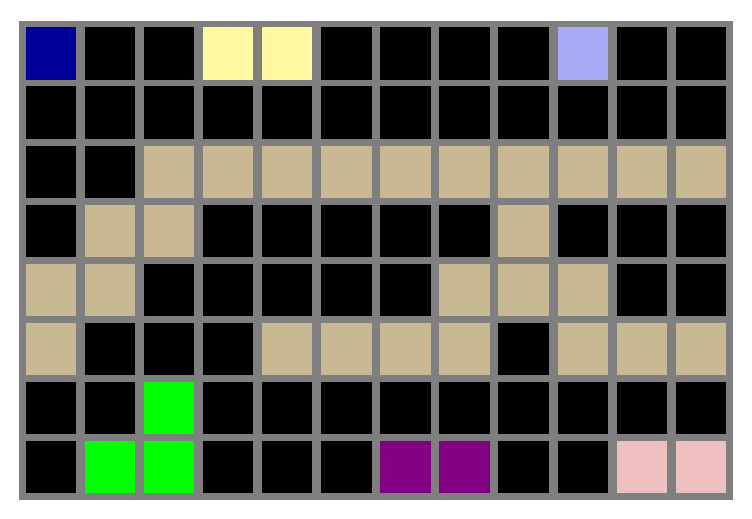
\includegraphics[width=\textwidth]{section-cumulos/motivacion-GMAP.eps}
        \caption{Matriz $\MATRIX{G}$ com valores inteiros, 
        representada como uma imagem com partículas (cúmulos) formados por grupos de pixels brancos.}
        \label{fig:motivacion-G}
    \end{subfigure}
\caption{Analisando partículas na matriz $\MATRIX{M}$.}
\label{fig:motivacion}
\end{figure}


A Figura \ref{fig:Diagrama} mostra um diagrama de bloco de um detetor de cúmulos,
o bloco recebe como entrada uma matriz binária $\MATRIX{M}$ e 
retorna uma matriz inteira $\MATRIX{G}\in \mathbb{N}^{N_l \times N_c}$, 
criada pela agrupação dos pixels brancos em cúmulos, como na Figura \ref{fig:motivacion-G}; onde 
todos os pixels num cúmulo são mapeados com o mesmo índice\footnote{Na 
figura cada diferente $id$ está representado com uma diferente cor.} 
$id$. % $\forall~0 \leq id \leq L$.
O identificador $id=0$ corresponde aos pixels pretos, é dizer os bits 0,
qualquer outro $id$ tomará um valor maior a zero.

\begin{figure}[!htb]
\centering
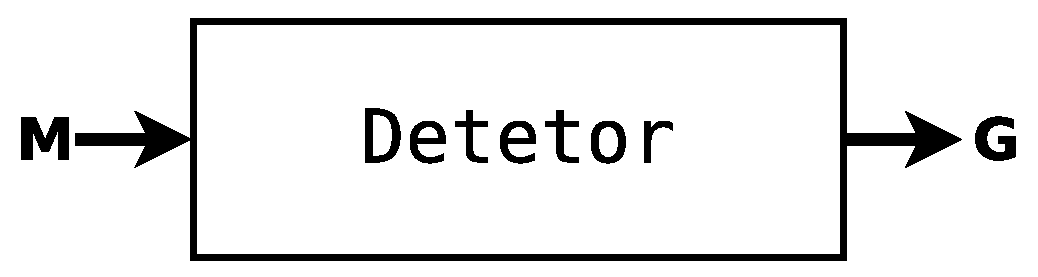
\includegraphics[width=0.35\textwidth]{section-cumulos/Diagrama.eps}
\caption{Diagrama de bloco do sistema.}
\label{fig:Diagrama}
\end{figure}



%%%%%%%%%%%%%%%%%%%%%%%%%%%%%%%%%%%%%%%%%%%%%%%%%%%%%%%%%%%%%%%%%%%%%%%%%%%%%%%%
\subsection{Detetor de cúmulos}
\label{subsec:part1}

Nosso problema principal é obter, a partir de uma matriz $\MATRIX{M}$, 
 uma matriz $\MATRIX{G}$ onde cada elemento contem
o índice do cúmulo ao qual pertence, como mostra a Figura \ref{fig:motivacion}.
Assim, pra cumprir este objetivo são usadas as funções $funA$ e $funB$, como mostra  a
Figura \ref{fig:modelocumulos}, onde são analisadas de maneira sequencial as colunas $\VECTOR{M}_c$ da
matriz $\MATRIX{M}$.
\begin{figure}[!htb]
\centering
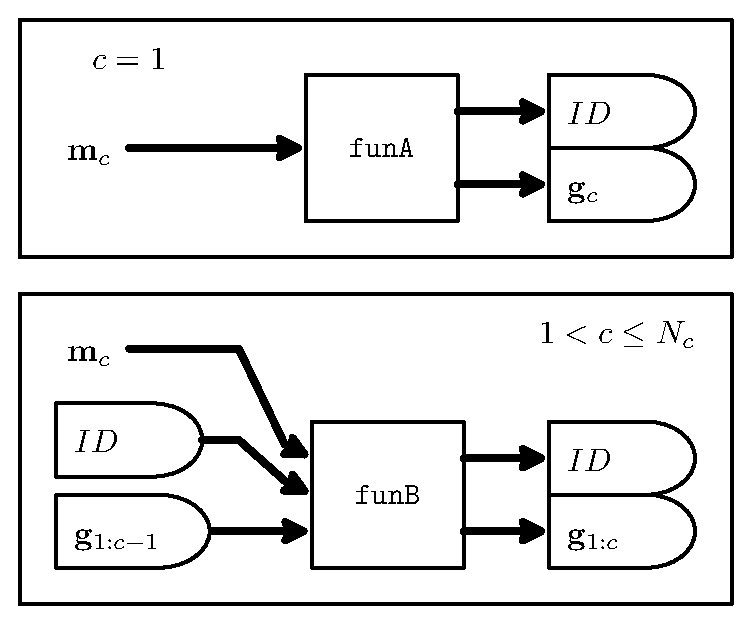
\includegraphics[width=0.45\textwidth]{section-cumulos/DiagramaCompleto.eps}
\caption{Diagrama de fluxo del algoritmo de criação de cúmulos.}
\label{fig:modelocumulos}
\end{figure}

\begin{itemize}
\item A função $funA$ recebe como parâmetro de entrada a coluna $\VECTOR{m}_1$ $\in\MATRIX{M}$.
Retorna o valor dos índices na coluna $\VECTOR{g}_1$ $\in\MATRIX{G}$;
adicionalmente a função retorna, $ID$, 
o valor do maior identificador $id$ atribuído aos cúmulos nas operações.

\item A função $funB$ recebe como parâmetros de entrada a $c$-ésima 
coluna $\VECTOR{m}_c$ $\in\MATRIX{M}$, o mapa de índices na submatriz $\VECTOR{g}_{1:(c-1)}$ $\in\MATRIX{G}$
que abrange informações de índice desde a primeira coluna ate a $(c-1)$-ésima e
$ID$ o valor do maior identificador $id$ atribuído aos cúmulos nas operações.
A função retorna a matriz $\VECTOR{g}_{1:c}$ com os dados dos índices desde a primeira coluna ate a $c$-ésima,
adicionalmente a função retorna o novo valor de $ID$.
\end{itemize}

%%%%%%%%%%%%%%%%%%%%%%%%%%%%%%%%%%%%%%%%%%%%%%%%%%%%%%%%%%%%%%%%%%%%%%%%%%%%%%%%
\subsubsection{Algoritmo da função $funA$}
\label{subsubsec:funA}
A função $funA$ recebe um vetor coluna $\VECTOR{m}_1$ com uns e zeros, como é exemplificado na
Figura \ref{fig:funA}, na saída a função retorna um vetor $\VECTOR{g}_1$ com o mesmo tamanho
porem com elementos com valores inteiros; este vetor representa o mapeamento dos índices $id$ em cada cumulo de $\VECTOR{m}_1$.
\begin{figure}[!htb]
\centering
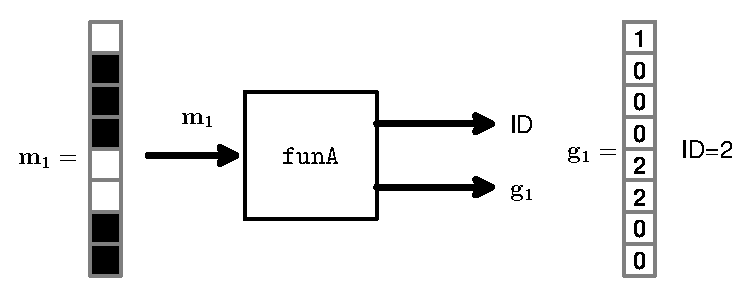
\includegraphics[width=0.7\textwidth]{section-cumulos/funA.eps}
\caption{Descrição da função $funA$.}
\label{fig:funA}
\end{figure}

Para calcular $\VECTOR{g}_1$ se usa o vetor $\VECTOR{m}_1$;
elementos com zero em $\VECTOR{m}_1$ provocam automaticamente elementos com um índice $0$ em $\VECTOR{g}_1$;
por outro lado, se achamos uma região de $1$'s em $\VECTOR{m}_1$, 
estes recebem em $\VECTOR{g}_1$ um mesmo índice,
sendo que cada região de $1$'s tem um índice diferente. 
A função $funA$ também retorna, $ID$, o máximo índice estabelecido em $\VECTOR{g}_1$.
Um algoritmo que explica este procedimento, pode ser visto no diagrama de fluxo da Figura \ref{fig:funA0};
o algoritmo usa a função $funB1$ copia zeros do vetor $\VECTOR{m}_1$ ao vetor $\VECTOR{g}_1$;
mais detalhes da função são explicados na Seção \ref{subsubsec:funB}.
\begin{figure}[!htb]
\centering
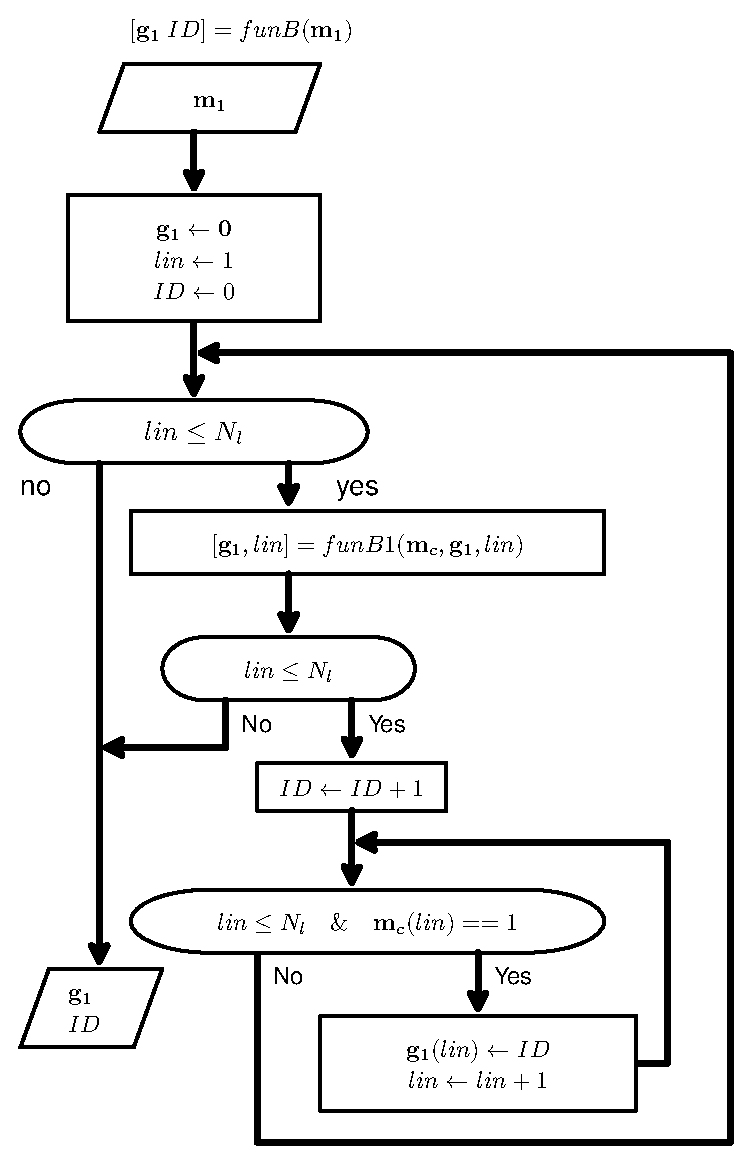
\includegraphics[width=0.5\textwidth]{section-cumulos/funA0.eps}
\caption{Descrição da função $funA$.}
\label{fig:funA0}
\end{figure}

%%%%%%%%%%%%%%%%%%%%%%%%%%%%%%%%%%%%%%%%%%%%%%%%%%%%%%%%%%%%%%%%%%%%%%%%%%%%%%%%
\subsubsection{Algoritmo da função $funB$}
\label{subsubsec:funB}
A função $funB$ recebe como parâmetros de entrada um vetor $\VECTOR{m}_{c}$, correspondente a 
$c$-ésima coluna da matriz $\MATRIX{M}$, a submatriz $\VECTOR{g}_{1:(c-1)}$ $\in\MATRIX{G}$ com o mapa de índices
desde a primeira coluna ate a $(c-1)$-ésima coluna da matriz $\MATRIX{G}$, 
e o máximo índice $ID$ nos elementos da matriz $\VECTOR{g}_{1:(c-1)}$. 
Na saída a função retorna uma matriz $\VECTOR{g}_{1:c}$ $\in\MATRIX{G}$ com o mapa de grupos
desde a primeira coluna ate a $c$-ésima coluna da matriz $\MATRIX{G}$, 
e o máximo índice $ID$ achado na matriz $\VECTOR{g}_{1:c}$.
A Figura \ref{fig:funB} mostra o diagrama fluxo do algoritmo da função $funB$.
\begin{figure}[!htb]
\centering
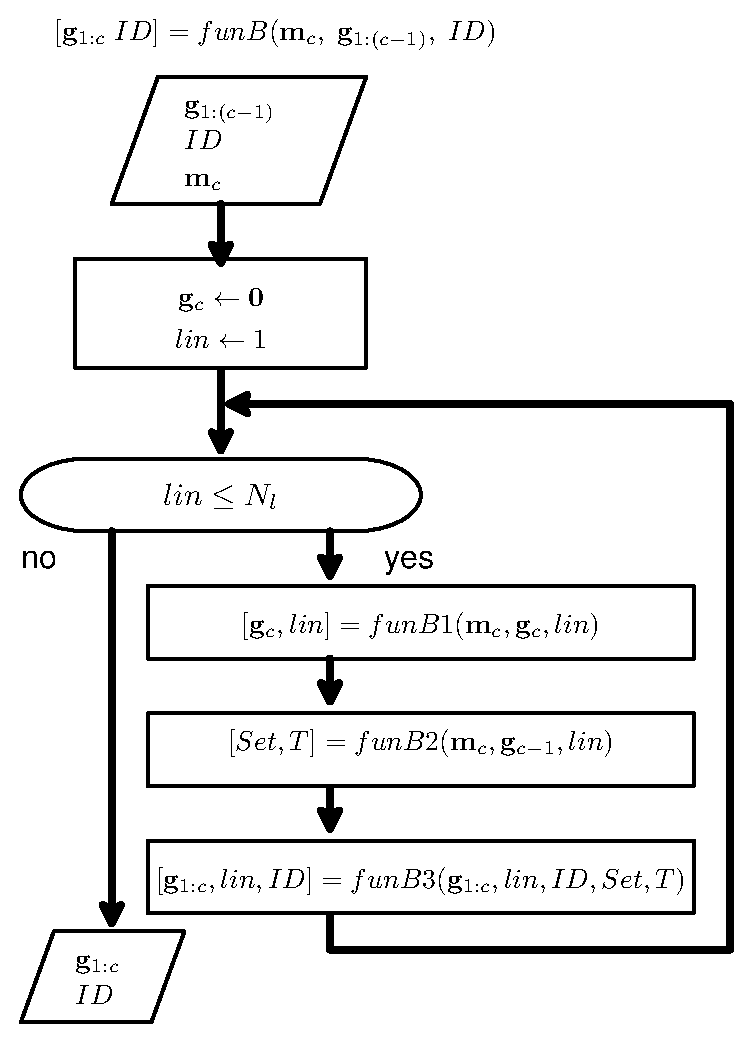
\includegraphics[width=0.45\textwidth]{section-cumulos/funB.eps}
\caption{Descrição da função $funB$ }
\label{fig:funB}
\end{figure}
A função $funB$ analisa os elementos do vetor $\VECTOR{m}_{c}$, desde o primeiro
elemento ate o elemento $N_l$; isto é realizado mediante as funções auxiliares $funB1$, $funB2$ e $funB3$,
de modo que estas funções modificam o conteúdo da matriz $\VECTOR{g}_{1:c}$ e a variável $ID$.

\textbf{Algoritmo da função $funB1$}:
A função recebe como parâmetros de entrada os vetores $\VECTOR{m}_{c}$, $\VECTOR{g}_{c}$
e uma variável com a linha $lin$ onde inciara o analises.
Se existem zeros no vetor $\VECTOR{m}_{c}$, então se escrevem zeros nos elementos na mesma posição 
no vetor $\VECTOR{g}_{c}$.
A função finaliza quando se acha o primeiro $1$ no vetor $\VECTOR{m}_{c}$,
carregando esta posição na variável $lin$, 
como mostra o diagrama de fluxo da Figura \ref{fig:funB1}.
\begin{figure}[!htb]
\centering
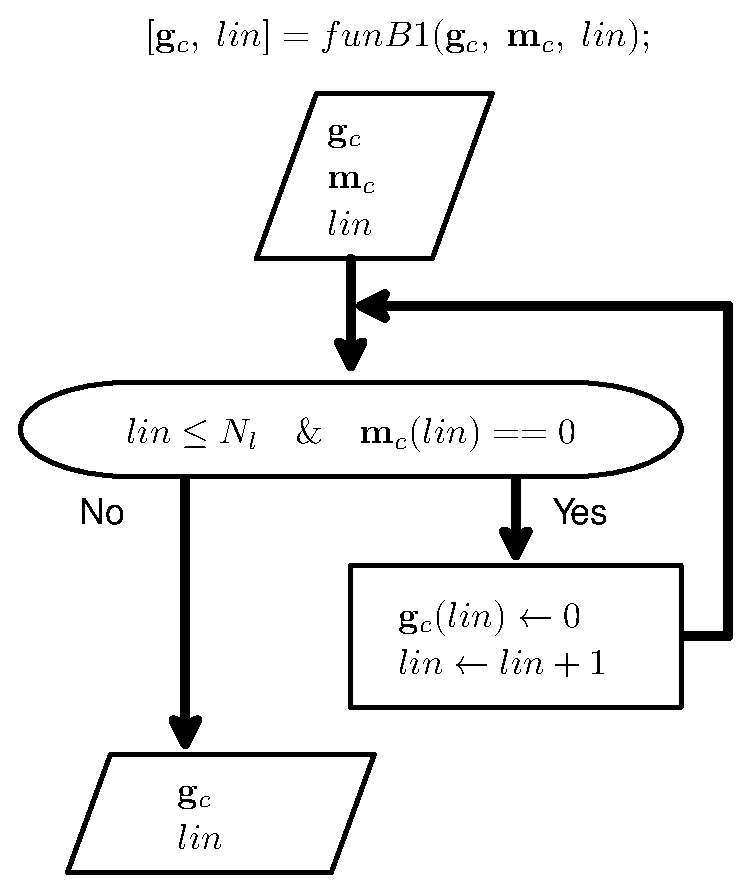
\includegraphics[width=0.45\textwidth]{section-cumulos/funB1.eps}
\caption{Descrição da função $funB1$ }
\label{fig:funB1}
\end{figure}

\textbf{Algoritmo da função $funB2$}:
A função recebe como parâmetros de entrada os vetores $\VECTOR{m}_{c}$, $\VECTOR{g}_{c-1}$
e uma variável com a linha $lin$ que indica a posição do primeiro $1$ achado com a função $funB1$. 
A função $funB2$ analisa somente um cumulo de $1$'s no vetor $\VECTOR{m}_{c}$, 
retornando um conjunto, $Set$, com os $id$'s no $\VECTOR{g}_{c-1}$ 
que estejam ao lado dos uns analisados no cúmulo em $\VECTOR{m}_{c}$;
adicionalmente a função $funB2$ retorna, $T$, o número de $1$'s do cúmulo.
O algoritmo da função $funB2$ pode ser visto no diagrama de fluxo da Figura \ref{fig:funB2};
nele podemos perceber o uso da função $Set.AddNoZero(id)$,
esta função agrega o índice $id$ ao conjunto $Set$,
se este ainda não existe em $Set$ e se $id\neq 0$.
\begin{figure}[!htb]
\centering
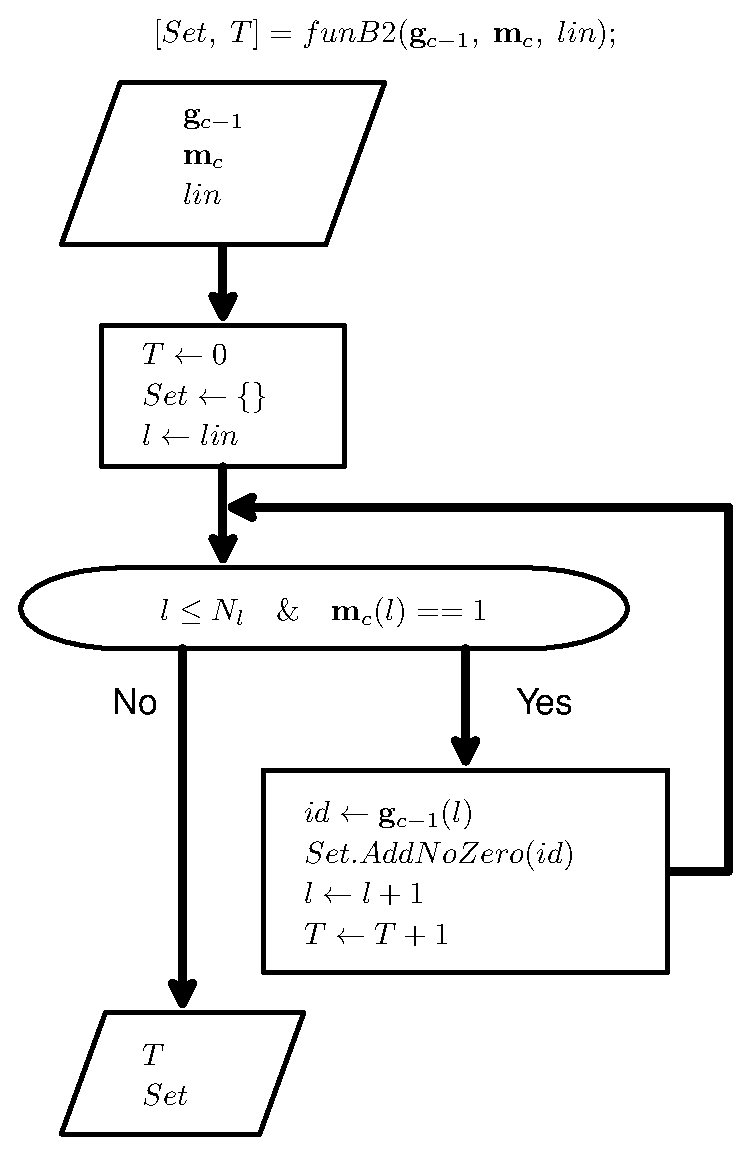
\includegraphics[width=0.45\textwidth]{section-cumulos/funB2.eps}
\caption{Descrição da função $funB2$ }
\label{fig:funB2}
\end{figure}

\textbf{Algoritmo da função $funB3$}:
A função recebe como parâmetros de entrada a submatriz $\VECTOR{g}_{1:c}$ $\in\MATRIX{G}$, 
uma variável com a linha $lin$ que indica a posição do primeiro $1$ achado com a função $funB1$,
o índice $ID$ que contem o valor do máximo $id$ nos elementos da submatriz $\VECTOR{g}_{1:(c-1)}$ $\in\MATRIX{G}$,
um conjunto $Set$ com todos os índice vizinhos ao cúmulo analisado com a função $funB2$,
e finalmente, $T$, o número de $1$'s no cúmulo.
A função $funB3$ se encarrega de escrever no vetor $\VECTOR{g}_{c}$ o índice correspondente,
e fusionar índices na submatriz $\VECTOR{g}_{1:(c-1)}$ se for necessário;
assim, a função retorna a submatriz $\VECTOR{g}_{1:c}$, com os índices modificados ate a $c$-ésima coluna 
e $lin$-ésima linha, também retorna o atual valor de $lin$ que indica o lugar do primeiro $0$ achado,
finalmente a função retorna o índice, $ID$, com maior valor achado na submatriz  $\VECTOR{g}_{1:c}$.
O algoritmo da função $funB3$ pode ser visto no diagrama de fluxo da Figura \ref{fig:funB3};
nele podemos perceber o uso da função $funC$,
esta função troca todos os índices $id$ em $\VECTOR{g}_{1:c-1}$, que existam no conjunto $Set$,
pelo valor do primeiro índice no conjunto $Set$, de modo que todo os elementos achados em 
$\VECTOR{g}_{1:c-1}$ tenham o índice $Set.at(1)$.
\begin{figure}[!htb]
\centering
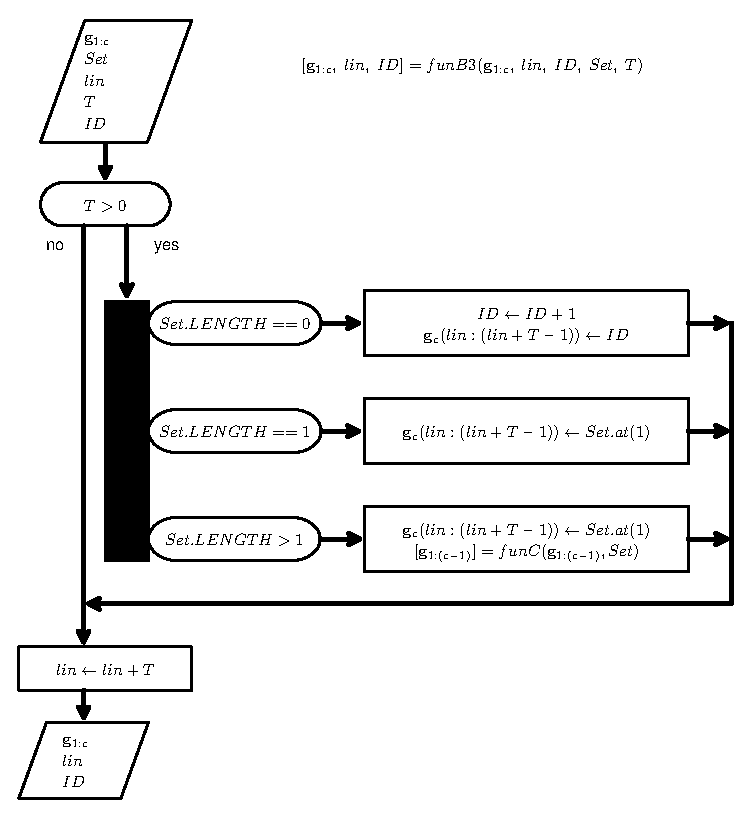
\includegraphics[width=0.65\textwidth]{section-cumulos/funB3.eps}
\caption{Descrição da função $funB3$ }
\label{fig:funB3}
\end{figure}

%%%%%%%%%%%%%%%%%%%%%%%%%%%%%%%%%%%%%%%%%%%%%%%%%%%%%%%%%%%%%%%%%%%%%%%%%%%%%%%%
%%%%%%%%%%%%%%%%%%%%%%%%%%%%%%%%%%%%%%%%%%%%%%%%%%%%%%%%%%%%%%%%%%%%%%%%%%%%%%%%
\subsection{Estatística da matriz $\MATRIX{G}$ }
\label{subsec:part1}


A informação em $\MATRIX{G}$ pode ser processada para 
retornar uma vetor $\VECTOR{s}$ com $L$ elementos, um por cada cúmulo,
onde $\VECTOR{s}(l)$ representa ao $l$-ésimo cúmulo analisado,
ver Figura \ref{fig:Diagrama2}.
Assim $\VECTOR{s}$ é uma estrutura que contem 
dados e estatística de cada cúmulo como:
\begin{itemize}
%\item Uma lista de todos os pixels no cúmulo com um identificador $id$.
\item $\VECTOR{s}(l).Id$ : O índice atribuído ao $l$-ésimo cúmulo.
\item $\VECTOR{s}(l).Area$ : A área em pixels do $l$-ésimo cúmulo.
%\item Centroide.
\end{itemize}


\begin{figure}[!htb]
\centering
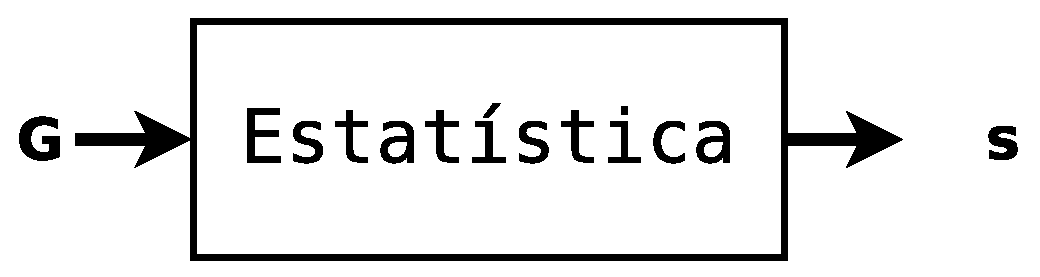
\includegraphics[width=0.35\textwidth]{section-cumulos/Diagrama2.eps}
\caption{Diagrama de bloco para obter estatística de $\MATRIX{G}$.}
\label{fig:Diagrama2}
\end{figure}



\clearpage
\newpage

\section{least-squares fitting of cubic splines}
\label{sec:spline3method1}

Aqui é mostrado como encaixar a curva $f(x):\mathbb{R}\rightarrow \mathbb{R}$, 
 sobre um conjunto de $N$ pontos $(x_n,y_n)$,
$\forall n \in \mathbb{Z},~0\leq n < N$; mediante o uso de mínimos quadrados, tendo
cada ponto uma importância de $w_n$.
Onde a curva 
$y=f(x)$ esta composta de um grupo de $M$ splines cúbicos (polinômios de grau 3), 
como o exemplo da Figura \ref{fig:leastmeanspline3}.
\begin{figure}[!htb]
\centering
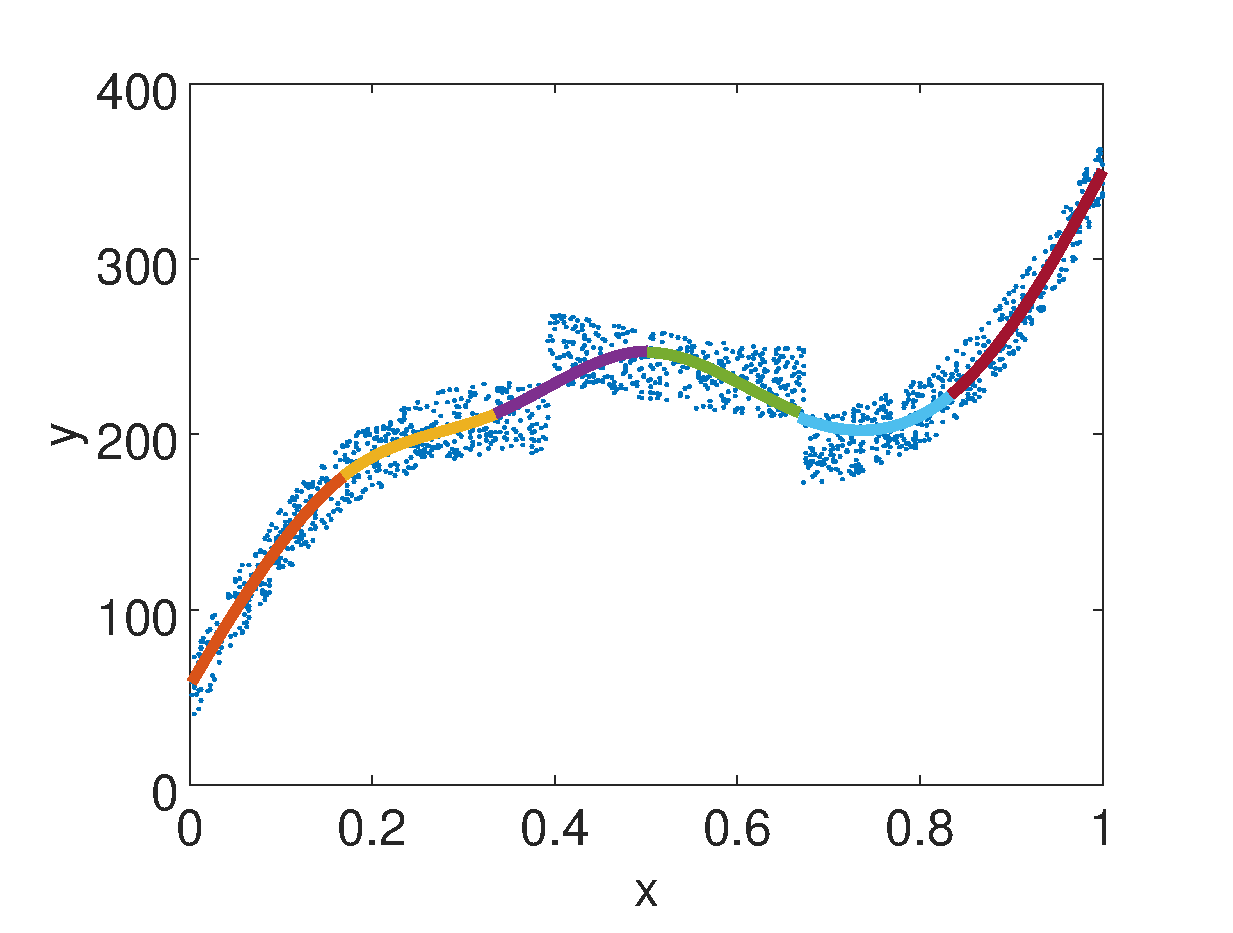
\includegraphics[width=0.6\textwidth]{section-cubic-splines/splines3demo.eps}
\caption{Encaixe de $M=6$ splines cúbicos num conjunto de $N=500$ pontos $\{x_n,y_n\}$.}
\label{fig:leastmeanspline3}
\end{figure}

Os splines tem seus limites de domínio, nas posições onde $x$ tem valores 
$d_{0}, d_{1}, d_{2}, ..., d_{M}$;
assim, podemos definir os vetores 
$\VECTOR{d}=\left(\begin{matrix}d_0 & d_1 & ...  & d_{M}\end{matrix}\right)^T$ $\in \mathbb{R}^{M+1}$ e
$\VECTOR{p}=\left(\begin{matrix}p_0 & p_1 & ...  & p_{4M-1}\end{matrix}\right)^T$ $\in \mathbb{R}^{4M}$,
de modo que podemos expressar $f(x)$ mediante
\begin{comment}
\begin{equation}
 G(x,a,b)= \left\{\begin{matrix}
1 & if &  a \leq x \leq b \\ 
0 & if & other~case
\end{matrix}\right.
\end{equation}
\end{comment}
o uso do polinômio cúbico
\begin{equation}
 S_k(x,\VECTOR{p})=P_{4k}~x^3+P_{1+4k}~x^2+P_{2+4k}~x+P_{3+4k},
\end{equation}
na função
\begin{comment}
\begin{equation}
 f(x,\VECTOR{p},\VECTOR{d})=\sum_{k=0}^{M-1} S_k(x,\VECTOR{p})G(x,d_{k},d_{k+1})  
\end{equation}
\end{comment}
\begin{equation}
f(x)\equiv f(x,\VECTOR{p},\VECTOR{d})= \left\{\begin{matrix}
S_0(x,\VECTOR{p}) & if & d_0 \leq x \leq d_1 \\ 
S_1(x,\VECTOR{p}) & if & d_1 \leq x \leq d_2 \\ 
S_2(x,\VECTOR{p}) & if & d_2 \leq x \leq d_3 \\ 
\vdots & \vdots & \vdots \\
S_{M-1}(x,\VECTOR{p}) & if & d_{M-1} \leq x \leq d_{M} \\  
\end{matrix}\right.
\end{equation}

%%%%%%%%%%%%%%%%%%%%%%%%%%%%%%%%%%%%%%%%%%%%%%%%%%%%%%%%%%%%%%%%%%%%%%%%%%%%%%%%
%%%%%%%%%%%%%%%%%%%%%%%%%%%%%%%%%%%%%%%%%%%%%%%%%%%%%%%%%%%%%%%%%%%%%%%%%%%%%%%%
\subsection{Calculando o vetor de parâmetros $\VECTOR{p}$}
Agrupando as $N$ amostras $\{x_n,y_n\}$ como mostrado na  Seção \ref{subsec:all}, 
podemos definir
\begin{equation}
\VECTOR{z}=
\left(\begin{matrix}
\VECTOR{y} \\
\mathbf{0} \\
\mathbf{0} \\
\mathbf{0} 
\end{matrix}\right),
\qquad 
\MATRIX{Q}=
\left(\begin{matrix}
\mathbf{A} \\
\MATRIX{B}_0 \\
\MATRIX{B}_1 \\
\MATRIX{B}_2 
\end{matrix}\right),
\qquad 
\MATRIX{R}=diag
\left(\begin{matrix}
\VECTOR{w} \\
\VECTOR{w}_a \\
\VECTOR{w}_b \\
\VECTOR{w}_c 
\end{matrix}\right);
\end{equation}
onde os vetores $\VECTOR{w}_a$, $\VECTOR{w}_b$ e $\VECTOR{w}_c$ são escolhido por nós,
e indicam o peso que desejamos dar ao cálculo do erro na continuidade de polinômios adjacentes,
na suas derivadas de ordem $0$, $1$ e $2$, respetivamente. 
Assim, para calcula o vetor $\VECTOR{p}$,  aplicamos $LMS$ (Least Mean Square)
definindo a  regra de minimização $e(\VECTOR{p}):\mathbb{R}^{4M}\rightarrow \mathbb{R}$,
\begin{equation}
 e(\VECTOR{p})=||\VECTOR{z} -\MATRIX{Q}  \VECTOR{p} ||_{\MATRIX{R}}^2+\alpha || \VECTOR{p}-\VECTOR{p}_{*} ||.
\end{equation}
Onde $\VECTOR{p}_{*}$ pode ser entendido como  $\VECTOR{p}$ numa iteração anterior; é dizer $\VECTOR{p}_{*}\equiv \VECTOR{p}_{k-1}$. Assim, aplicando
$LMS$ e a regularização de Tikhonov, o mínimo valor de $\VECTOR{p}=\VECTOR{\hat{p}}$ que minimiza $e(\VECTOR{p})$ 
se obtêm iterativamente usando a equação
\begin{equation}
\VECTOR{p}_{k}= \VECTOR{p}_{k-1}+ \left[ \MATRIX{Q}^T \MATRIX{R}\MATRIX{Q} +\alpha \mathbf{I} \right]^{-1} \MATRIX{Q}^T \MATRIX{R}  \left[ \VECTOR{z}-\MATRIX{Q}  \VECTOR{p}_{k-1} \right]
\end{equation}
desde um $\VECTOR{p}_{0}$ sabiamente escolhido,
ate que os vetores $\VECTOR{p}_{k}$ e $\VECTOR{p}_{k-1}$ sejam muito próximos,
onde se declara que $\VECTOR{\hat{p}}=\VECTOR{p}_{k}$. 



%%%%%%%%%%%%%%%%%%%%%%%%%%%%%%%%%%%%%%%%%%%%%%%%%%%%%%%%%%%%%%%%%%%%%%%%%%%%%%%%
%%%%%%%%%%%%%%%%%%%%%%%%%%%%%%%%%%%%%%%%%%%%%%%%%%%%%%%%%%%%%%%%%%%%%%%%%%%%%%%%
\subsection{Modelando a solução}
\label{subsec:all}
Para poder calcular o vetor $\VECTOR{p}=\left(\begin{matrix}p_0 & p_1 & p_2 & ...  & p_{4M-1}\end{matrix}\right)^T$, 
do problema spline descrito  na Seção \ref{sec:spline3method1}, a partir dos dados $(x_n,y_n,w_n)$; 
$\forall n \in \mathbb{Z},~0\leq n < N$,
é necessário escolher os valores $\VECTOR{d}=\left(\begin{matrix}d_0 & d_1 & ...  & d_{M}\end{matrix}\right)^T$;
ordenamos nossos dados nos seguintes vetores e sub-vetores coluna:
\begin{equation}
\VECTOR{x}=\left(\begin{matrix}\VECTOR{x}_0 \\ \VECTOR{x}_1 \\ \vdots  \\ \VECTOR{x}_{m}\\ \vdots  \\ \VECTOR{x}_{M-1}\end{matrix}\right),~~
\VECTOR{y}=\left(\begin{matrix}\VECTOR{y}_0 \\ \VECTOR{y}_1 \\ \vdots  \\ \VECTOR{y}_{m}\\ \vdots  \\ \VECTOR{y}_{M-1}\end{matrix}\right),~~
\VECTOR{w}=\left(\begin{matrix}\VECTOR{w}_0 \\ \VECTOR{w}_1 \\ \vdots  \\ \VECTOR{w}_{m}\\ \vdots  \\ \VECTOR{w}_{M-1}\end{matrix}\right),
\end{equation}
onde $\VECTOR{x}$, $\VECTOR{y}$ e  $\VECTOR{z}$ $\in \mathbb{R}^{N}$, e os sub-vetoes $\VECTOR{x}_m$, $\VECTOR{y}_m$ e $\VECTOR{w}_m$, incluem informação de $\{x_n,y_n,w_n\}$
que tem  domínio em $d_{m} \leq x_n \leq d_{m+1}$.


\subsubsection{Minimização do erro  $||\VECTOR{y} - \mathbf{A}\VECTOR{p}||^2_{\MATRIX{W}}$}
\label{subsubsec:partz}
Os dados $(x_n,y_n)$ são agrupados de forma que se procura minimizar $||\VECTOR{y} - \mathbf{A}\VECTOR{p}||^2_{\MATRIX{W}}$, 
onde a matriz diagonal $\MATRIX{W}=diag(\VECTOR{w})$,
\begin{equation}
\mathbf{A}_m =\left(\begin{matrix}
\VECTOR{x}_m^3 & \VECTOR{x}_m^2 & \VECTOR{x}_m & \mathbf{1}
\end{matrix}\right)
\end{equation}
\begin{equation}
\mathbf{A} =\left(\begin{matrix}
\mathbf{A}_0 & \mathbf{0}   & \mathbf{0}   & \dots & \mathbf{0} \\
\mathbf{0}   & \mathbf{A}_1 & \mathbf{0}   & \dots & \mathbf{0} \\
\mathbf{0}   & \mathbf{0}   & \mathbf{A}_2 & \dots & \mathbf{0} \\
\mathbf{0}   & \mathbf{0}   & \mathbf{0}   & \dots & \mathbf{A}_{M-1} \\
\end{matrix}\right) \in \mathbb{R}^{N \times 4M}
\end{equation}

\subsubsection{Minimização do erro $||\MATRIX{B}_0\VECTOR{p}||^2_{\MATRIX{W}_a}$ na derivada de ordem $0$ em splines adjacentes}
\label{subsubsec:part0}
Dados os polinômios $S_{k-1}(x,\VECTOR{p})$ e $S_{k}(x,\VECTOR{p})$ do $(k-1)$-ésimo e $k$-ésimo spline,
respetivamente. Podemos igualar ambos polinômios para garantir a continuidade dos splines em $x=d_{k}$, 
de modo que,
\begin{equation}
 S_{k-1}(d_{k},\VECTOR{p})=S_{k}(d_{k},\VECTOR{p}),
\end{equation}
Se agrupamos estas equações para os valores de  $0<k<M$, obtemos o sistema $\mathbf{0}=\MATRIX{B}_0 \VECTOR{p}$, 
onde $\MATRIX{B}_0 \in \mathbb{R}^{M-1 \times 4M}$ é definido como
\begin{equation}
\MATRIX{B}_0 =\left(\begin{matrix}
\VECTOR{e}_1 & -\VECTOR{e}_1   & \mathbf{0}    &  \mathbf{0}   & \dots & \mathbf{0} & \mathbf{0}\\
\mathbf{0}   &  \VECTOR{e}_2   & -\VECTOR{e}_2 &  \mathbf{0}   & \dots & \mathbf{0} & \mathbf{0}\\
\mathbf{0}   &  \mathbf{0}     &  \VECTOR{e}_3 & -\VECTOR{e}_3 & \dots & \mathbf{0} & \mathbf{0}\\
\vdots       &  \vdots         &  \vdots       &  \vdots       & \dots & \vdots     & \vdots\\
\mathbf{0}   &  \mathbf{0}     &  \mathbf{0}   &  \mathbf{0}   & \dots & \VECTOR{e}_{M-1} & -\VECTOR{e}_{M-1} \\
\end{matrix}\right),
\end{equation}
usando como variável auxiliar, 
\begin{equation}
\VECTOR{e}_k =\left(\begin{matrix}
d^3_k & d^2_k   & d_k & 1  \\
\end{matrix}\right).
\end{equation}
Assim neste caso é interessante minimizar a função de custo $||\MATRIX{B}_0\VECTOR{p}||^2_{\MATRIX{W}_a}$,
onde a matriz diagonal $\MATRIX{W}_a=diag(\VECTOR{w}_a)$ é escolhido por nos, 
mas é recomendável que $\VECTOR{w}_a$ tenha o mesmo peso que $\VECTOR{w}$,
pelo que poderíamos escolher $\VECTOR{w}_a=\frac{sum(\VECTOR{w})}{M-1}[1 1 1 ... 1]^T$
\subsubsection{Equação de continuidade da 1ra derivada dos splines consecutivos}
\label{subsubsec:part1}
Dados os polinômios $S_{k-1}(x,\VECTOR{p})$ e $S_{k}(x,\VECTOR{p})$ do $(k-1)$-ésimo e $k$-ésimo spline,
respetivamente. Podemos igualar a primeira derivada de  ambos polinômios para garantir a continuidade dos splines em $x=d_{k}$, 
de modo que,
\begin{equation}
 \left.\frac{\partial~S_{k-1}(x,\VECTOR{p})}{\partial x}\right|_{x=d_{k}} = 
 \left.\frac{\partial~S_{k}  (x,\VECTOR{p})}{\partial x}\right|_{x=d_{k}}
\end{equation}
Assim, agrupando as equações dos polinômios de  $0<k<M$, obtemos $\mathbf{0}=\MATRIX{B}_1 \VECTOR{p}$, onde,
\begin{equation}
\MATRIX{B}_1 =\left(\begin{matrix}
\partial\VECTOR{e}_1 & -\partial\VECTOR{e}_1   & \mathbf{0}    &  \mathbf{0}   & \dots & \mathbf{0} & \mathbf{0}\\
\mathbf{0}   &  \partial\VECTOR{e}_2   & -\partial\VECTOR{e}_2 &  \mathbf{0}   & \dots & \mathbf{0} & \mathbf{0}\\
\mathbf{0}   &  \mathbf{0}     &  \partial\VECTOR{e}_3 & -\partial\VECTOR{e}_3 & \dots & \mathbf{0} & \mathbf{0}\\
\vdots       &  \vdots         &  \vdots       &  \vdots       & \dots & \vdots     & \vdots\\
\mathbf{0}   &  \mathbf{0}     &  \mathbf{0}   &  \mathbf{0}   & \dots & \partial\VECTOR{e}_{M-1} & -\partial\VECTOR{e}_{M-1} \\
\end{matrix}\right),
\end{equation}
usando como variável auxiliar,
\begin{equation}
\partial\VECTOR{e}_k =\left(\begin{matrix}
3d^2_k & 2d_k   & 1 & 0  \\
\end{matrix}\right).
\end{equation}

\subsubsection{Equação de continuidade da 2da derivada dos splines consecutivos}
\label{subsubsec:part2}
Dados os polinômios $S_{k-1}(x,\VECTOR{p})$ e $S_{k}(x,\VECTOR{p})$ do $(k-1)$-ésimo e $k$-ésimo spline,
respetivamente. Podemos igualar a segunda derivada de ambos polinômios para garantir a continuidade dos splines em $x=d_{k}$, 
de modo que,
\begin{equation}
 \left.\frac{\partial^2~S_{k-1}(x,\VECTOR{p})}{\partial x^2}\right|_{x=d_{k}} = 
 \left.\frac{\partial^2~S_{k}  (x,\VECTOR{p})}{\partial x^2}\right|_{x=d_{k}}
\end{equation}
Assim, agrupando as equações dos polinômios de  $0<k<M$, obtemos $\mathbf{0}=\MATRIX{B}_2 \VECTOR{p}$, onde,
\begin{equation}
\MATRIX{B}_2 =\left(\begin{matrix}
\partial^2\VECTOR{e}_1 & -\partial^2\VECTOR{e}_1   & \mathbf{0}    &  \mathbf{0}   & \dots & \mathbf{0} & \mathbf{0}\\
\mathbf{0}   &  \partial^2\VECTOR{e}_2   & -\partial^2\VECTOR{e}_2 &  \mathbf{0}   & \dots & \mathbf{0} & \mathbf{0}\\
\mathbf{0}   &  \mathbf{0}     &  \partial^2\VECTOR{e}_3 & -\partial^2\VECTOR{e}_3 & \dots & \mathbf{0} & \mathbf{0}\\
\vdots       &  \vdots         &  \vdots       &  \vdots       & \dots & \vdots     & \vdots\\
\mathbf{0}   &  \mathbf{0}     &  \mathbf{0}   &  \mathbf{0}   & \dots & \partial^2\VECTOR{e}_{M-1} & -\partial^2\VECTOR{e}_{M-1} \\
\end{matrix}\right),
\end{equation}
usando como variável auxiliar,
\begin{equation}
\partial^2\VECTOR{e}_k =\left(\begin{matrix}
6d_k & 2   & 0 & 0  \\
\end{matrix}\right).
\end{equation}






%----------------------------------------------------------------------------------------
%	REFERENCE LIST
%----------------------------------------------------------------------------------------

\printbibliography

\end{document}
